\section{Modelo de Banco de Dados} % ### 5.4. Modelo de Banco de Dados

Considerando as informações necessárias para o presente trabalho, e também o preparo de campo para potenciais aplicações futuras, foi elaborado um diagrama conceitual de banco de dados, que pode ser visto na Figura \ref{fig:DiagramConceitual}.

\begin{figure}[htbp]\centering
  \caption{\label{fig:DiagramConceitual} Diagrama Conceitual do banco de dados}
  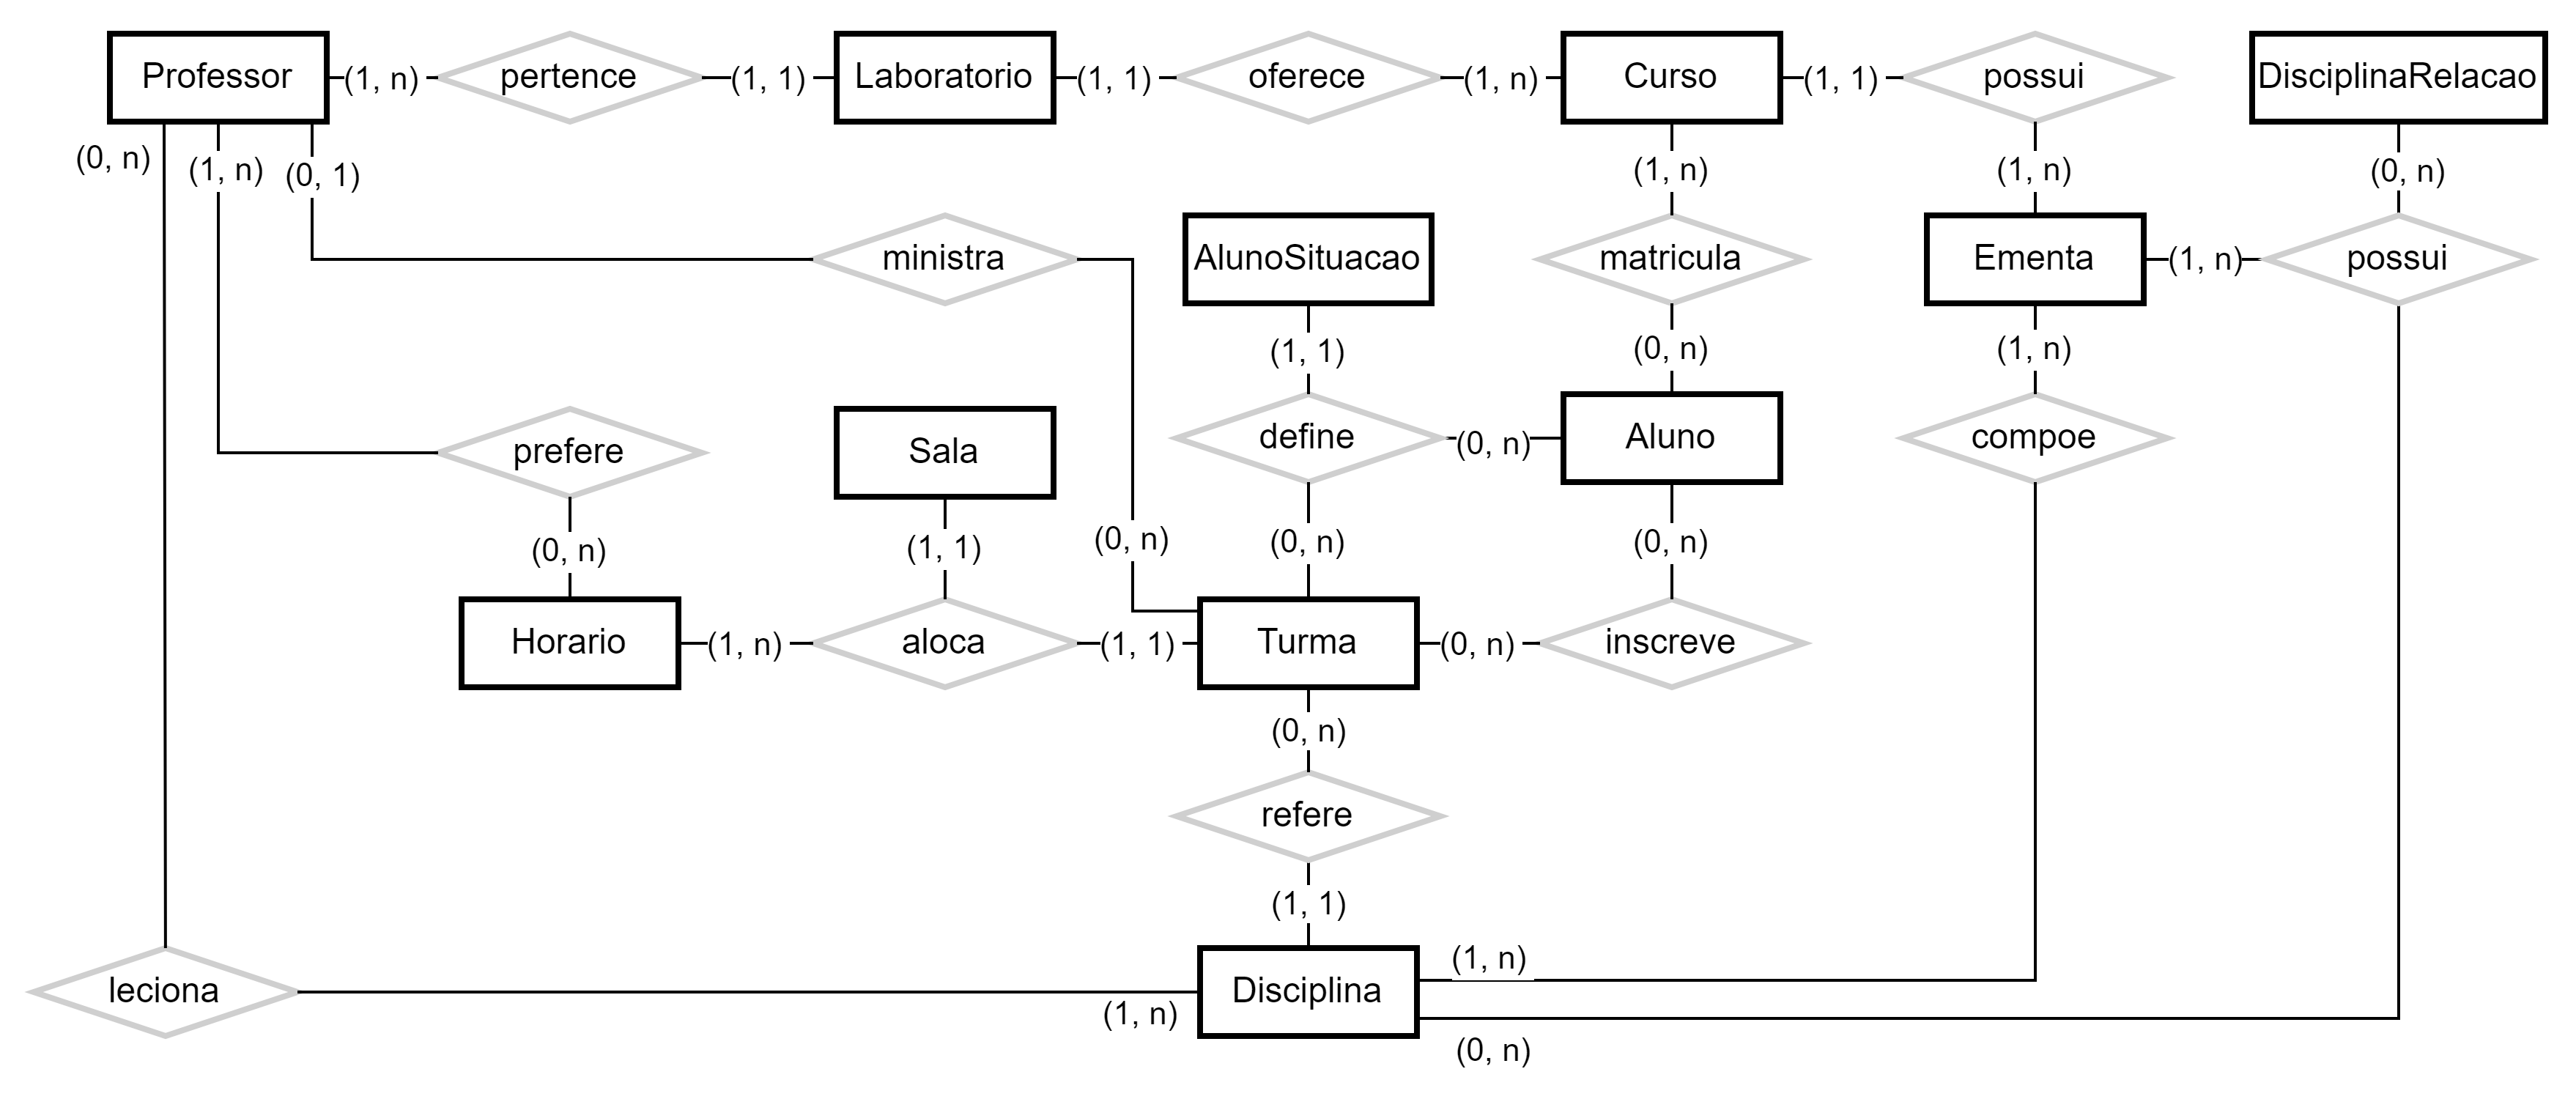
\includegraphics[scale=0.2]{files/img/DiagramaConceitual/DiagramaConceitualBranco.png}
  \legend{Fonte: o autor}
\end{figure} % Diagrama Conceitual

O diagrama conceitual foi elaborado utilizando a ferramenta \href{https://www.drawio.com/}{draw.io} citada na metodologia e ilustra as relações entre diversas entidades presentes na realidade da UENF. O emaranhamento presente no diagrama ilustra a complexidade envolvida na criação de uma grade horária, onde diversas entidades se relacionam entre si.

Como principais apontamentos, podemos citar a parte principal do modelo que é a alocação de turmas. Ela, como já descrito, envolve a correlação entre alunos de diferentes cursos, professores, disciplinas, salas e horários. Além disso, também é possível notar a presença de entidades que não são diretamente relacionadas à alocação de turmas, mas que podem se mostrar úteis, como a relação entre professores e laboratórios, e a de disciplinas e ementas.

\section{Desenvolvimento Web} % ### 5.5. Desenvolvimento Web <!-- Entrar em contato com a GINFO -->

Como forma de disponibilizar o acesso online, desenvolveu-se então, com os modelos elaborados um website utilizando do framework \href{https://react.dev/}{React}.

Buscou-se utilizar uma máquina virtual disponibilizada pela própria UENF, para evitar que houve problemas de conexão por parte dos servidores que em sua rede estivessem conectados.

O bando de dados utilizado foi o \href{https://dev.mysql.com/}{MySQL}, visto que é o mesmo utilizado pelo Sistema Acadêmico, assim proporcionando uma possível maior facilidade em uma hipotética integração futura.

